\subsection{Aufgabe 1}
Um die Laufzeit der Schallgeschwindigkeit in Luft zu messen, verbanden wir eine Klatsche mit einem Mikrophon. Das Mikrophon war wiederum mit einem Speicheroszilloskop verbunden, welches die gesammelten Daten an den Computer sendete. Auf dem Rechner wurden anschließend die Daten mit dem Programm PCS100 aufgezeichnet.\\
Gestartet wurde die Messung durch den Impuls, welcher von der Klatsche über ein Kabel zum Mikrophon gesendet wird.\\
Die verschiedenen Abstände zwischen dem Mikrophon und der Klatsche werden in der folgenden Tabelle 1 dargestellt. Um möglichst genaue Messwerte zu erhalten, führten wir jede Messung zweimal durch und bildeten den Mittelwert aus den Werten des ersten Schallimpulses. Das Programm des Computers lieferte uns Bilder wie in Abbildung 1 dargestellt. Wir benutzten aber die Werte der dazugehörigen Textdokumente, um den Zeitpunkt der Ankunft der ersten Schallwelle zu bestimmen.
\\
\begin{center}
\begin{minipage}{\linewidth}
\centering
\makebox[0cm]{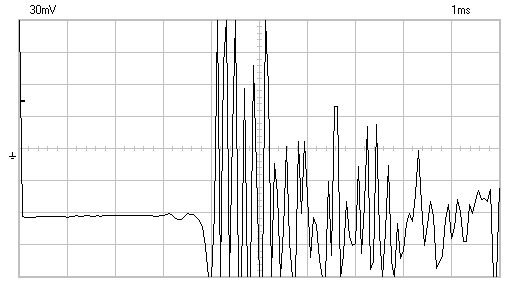
\includegraphics[width=\textwidth]{graphen/a1/100_1.png}}
\captionof{figure}{Beispielhafte Ausgabe des Programms PCS100}
\end{minipage}
\label{test}
\end{center}

\begin{center}
\begin{tabular}{|c|c|c|}
Abstand l [m] & Zeit t [ms] & Schallgeschwindigkeit c [\(\frac{m}{s}\)]\\
\hline
\(1.00 \pm 0.05\) & \(3.18 \pm 0.10\) & \(314.47 \pm 9.89\)\\
\(1.10 \pm 0.05\) & \(3.24 \pm 0.10\) & \(339.51 \pm 10.48\)\\
\(1.12 \pm 0.05\) & \(3.72 \pm 0.10\) & \(322.58 \pm 8.68\)\\
\(1.30 \pm 0.05\) & \(3,95 \pm 0.10\) & \(329.12 \pm 8.34\)\\
\(1.40 \pm 0.05\) & \(4.01 \pm 0.10\) & \(349.13 \pm 8.71\)\\
\(1.50 \pm 0.05\) & \(4.26 \pm 0.10\) & \(352.12 \pm 8.27\)\\
\(1.60 \pm 0.05\) & \(4.54 \pm 0.10\) & \(352.43 \pm 7.78\)\\
\(1.70 \pm 0.05\) & \(4.71 \pm 0.10\) & \(360.94 \pm 7.67\)\\
\(1.80 \pm 0.05\) & \(4.77 \pm 0.10\) & \(370.37 \pm 7.92\)\\
\(1.90 \pm 0.05\) & \(5.45 \pm 0.10\) & \(348.63 \pm 6.40\)\\
\hline
\end{tabular}
\captionof{table}{Messung der Schallgeschwindigkeit in Luft}
\end{center}

Die Schallgeschwindigkeit wir über die Relation \(c=\frac{l}{t}\) berechnet. Den Fehler erhalten wir über die Gauß'sche Fehlerfortpflanzung
\begin{equation}
\notag
\Delta c_i = \sqrt{\left(\frac{\partial c_i}{\partial l}\right)^2\cdot \left(\Delta l\right)^2+\left(\frac{\partial c_i}{\partial t}\right)^2\cdot \left(\Delta t\right)^2}=\sqrt{\frac{1}{t^2}\left(\Delta s\right)^2+\frac{s^2}{t^4}\left(\Delta t\right)^2}
\end{equation}
Für die gemittelte Schallgeschwindigkeit ergibt sich einen Wert von\\
\(\overline{c}=(343.93 \pm 5.53)\frac{m}{s}\)

Der Fehler des Mittelwerts errechnet sich aus der Standartabweichung des Mittelwerts:

\begin{equation}
\Delta c=\sqrt{\frac{\sum (c_i-\overline{c})^2}{n(n-1)}}
\end{equation}

Um den Wert von \(\overline{c}\) zu prüfen, vergleichen wir ihn mit dem Literaturwert, welcher in trockener Luft 343\(\frac{m}{s}\) entspricht. Damit ist der Wert identisch.

\subsection{Fazit}
Die Messung für diesen Versuch verlief ohne weitere Komplikationen. Der Errechnete Wert der Schallgeschwindigkeit ist absolut identisch mit dem Literaturwert, womit wir diese Aufgabe als gelöst anerkennen können.